
\chapter{Concept Model}
\label{chap:lu.uni.lassy.excalibur.group09.spec-CM}


\section{PrimaryTypes-Classes}
\subsection{Local view 12}
\label{sec:lu.uni.lassy.excalibur.group09.spec-CM-view-local-PrimaryTypes-Classes-12}
Figure \ref{fig:lu.uni.lassy.excalibur.group09.spec-CM-view-local-PrimaryTypes-Classes-12} Main view of the concept model



\begin{figure}[htbp] 
\label{fig:lu.uni.lassy.excalibur.group09.spec-CM}
\begin{center}
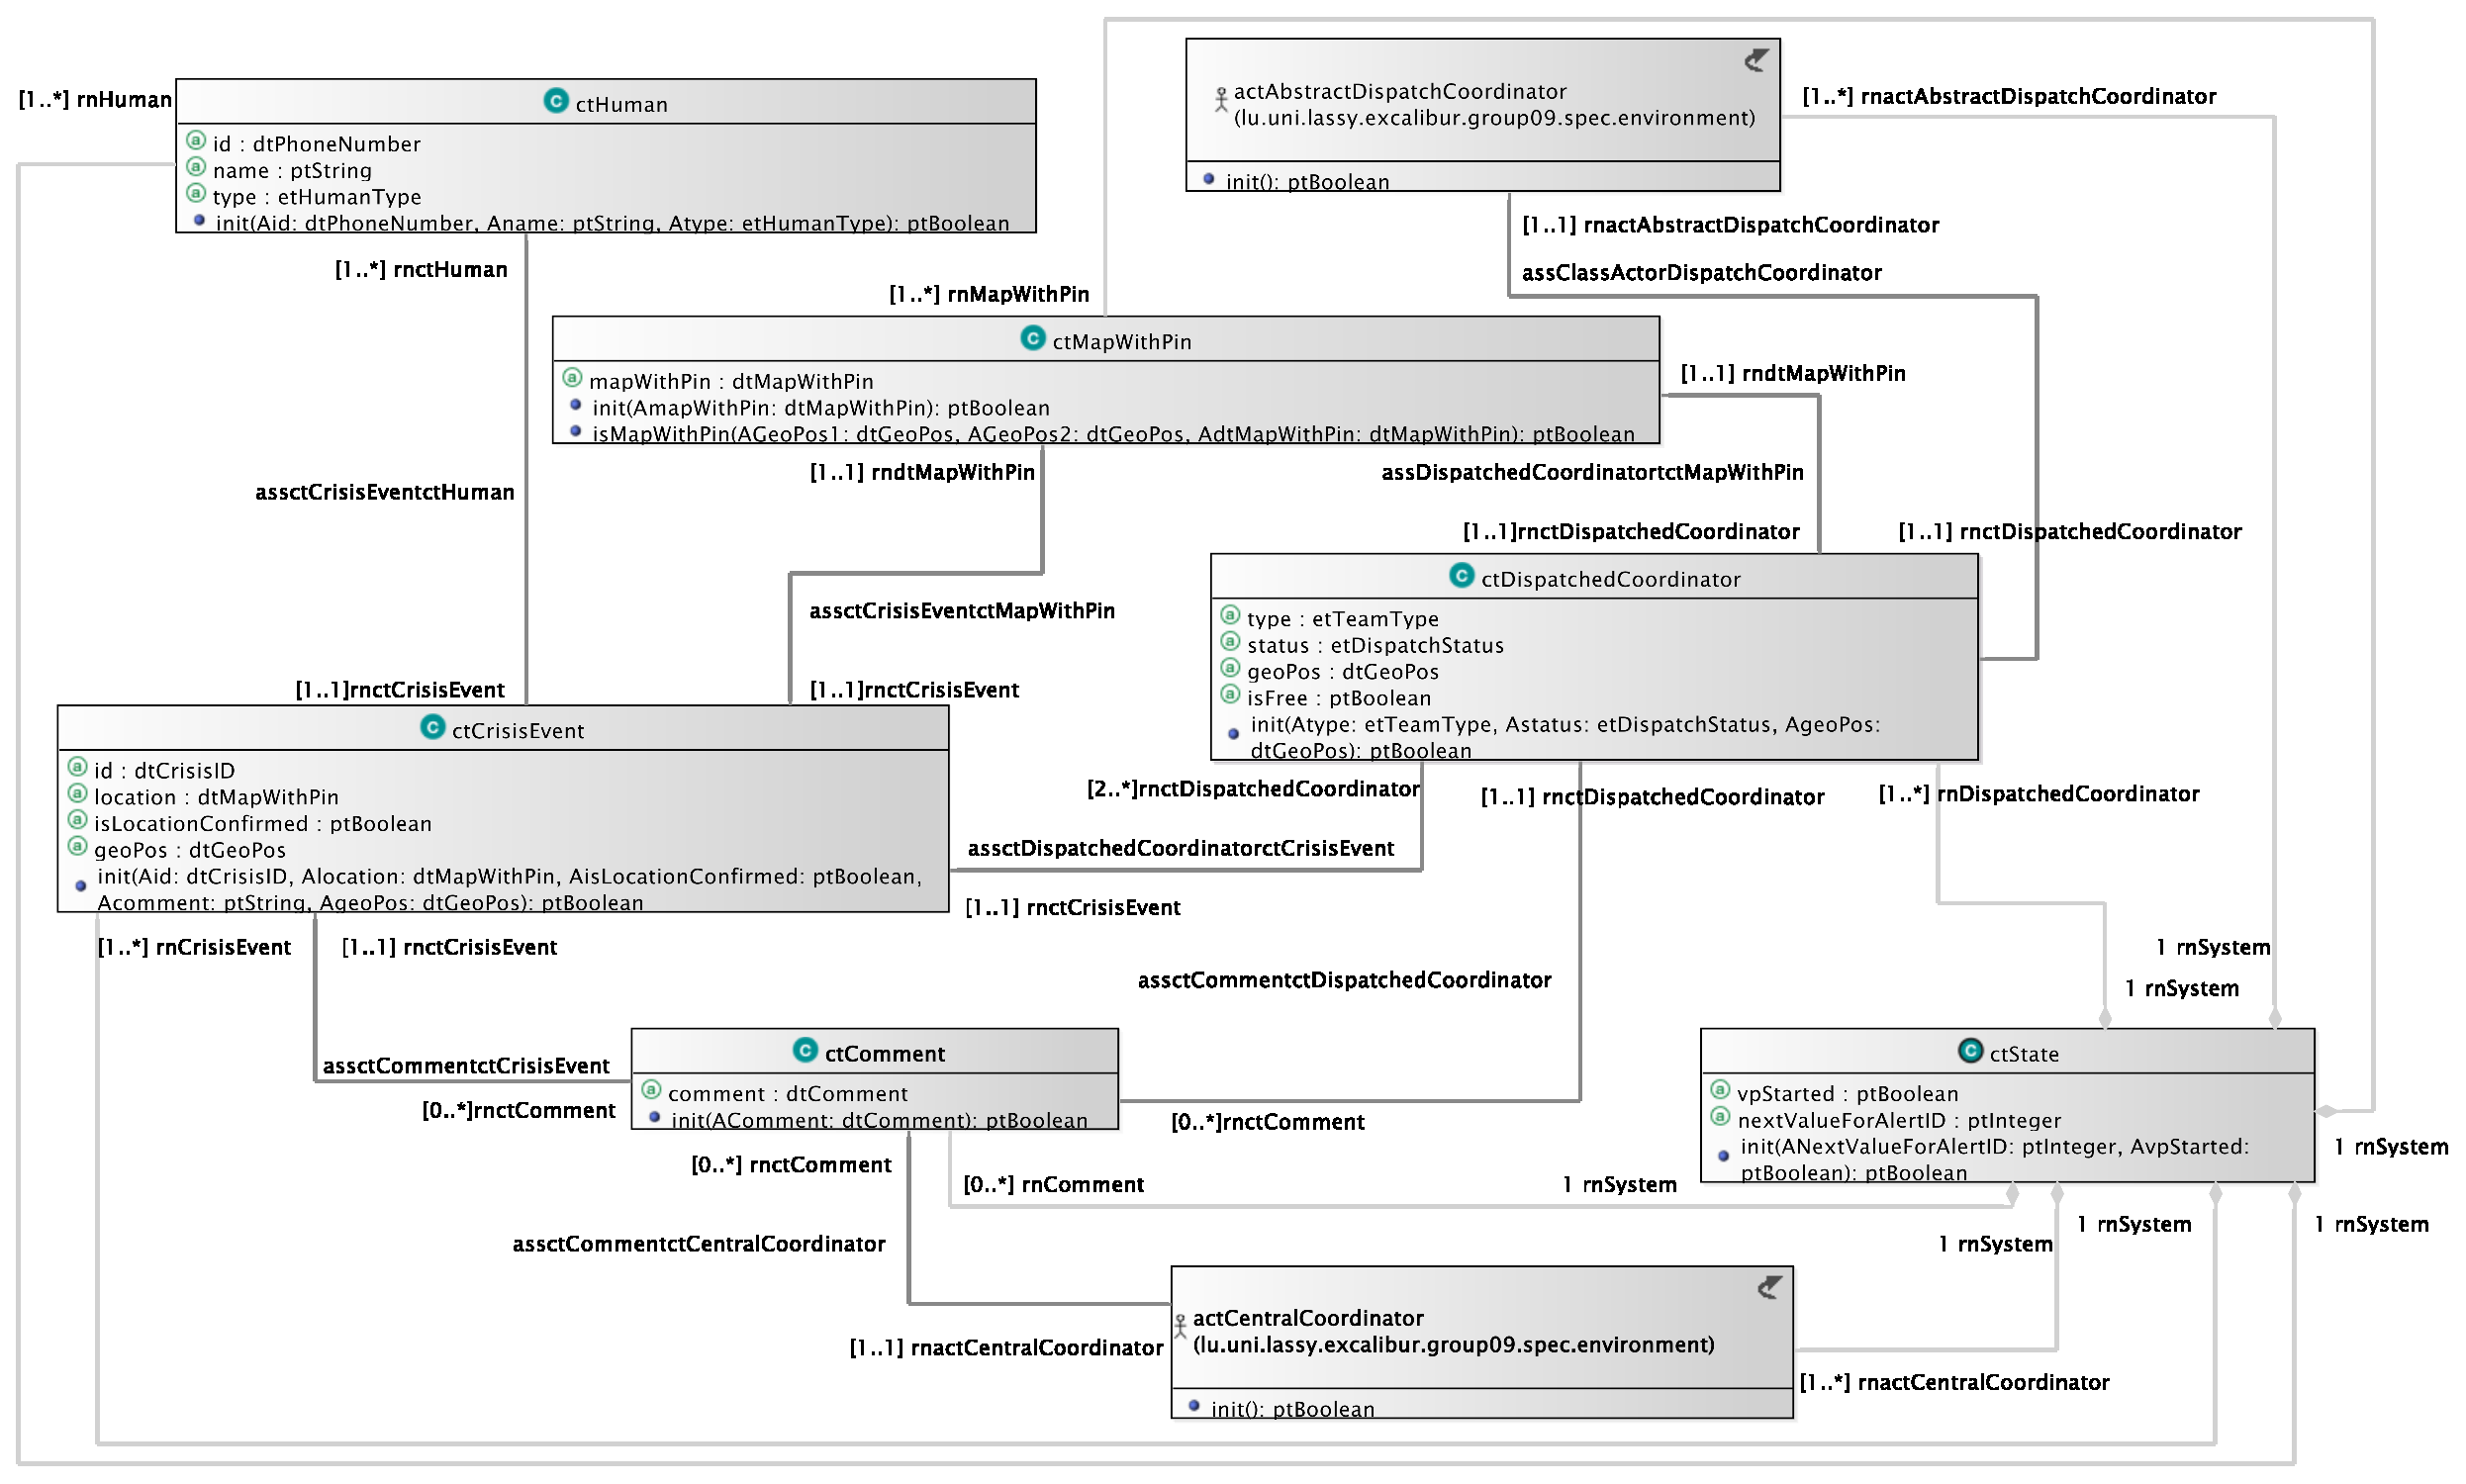
\includegraphics[
angle=90
,height=1.0\textheight
]{./images-report-gen/concept-model/local/PrimaryTypes-Classes/12/cm-ctAssociations.eps}
\end{center}
\caption[Concept Model - PrimaryTypes-Classes local view 12 - Main view of the concept model]{Concept Model - PrimaryTypes-Classes local view 12. Main view of the concept model.}
\label{fig:lu.uni.lassy.excalibur.group09.spec-CM-view-local-PrimaryTypes-Classes-12}
\end{figure}
\vspace{0.5cm} 




\section{PrimaryTypes-Datatypes}
\subsection{Local view 15}
\label{sec:lu.uni.lassy.excalibur.group09.spec-CM-view-local-PrimaryTypes-Datatypes-15}
Figure \ref{fig:lu.uni.lassy.excalibur.group09.spec-CM-view-local-PrimaryTypes-Datatypes-15} View of all the datatypes



\begin{figure}[htbp] 
\label{fig:lu.uni.lassy.excalibur.group09.spec-CM}
\begin{center}
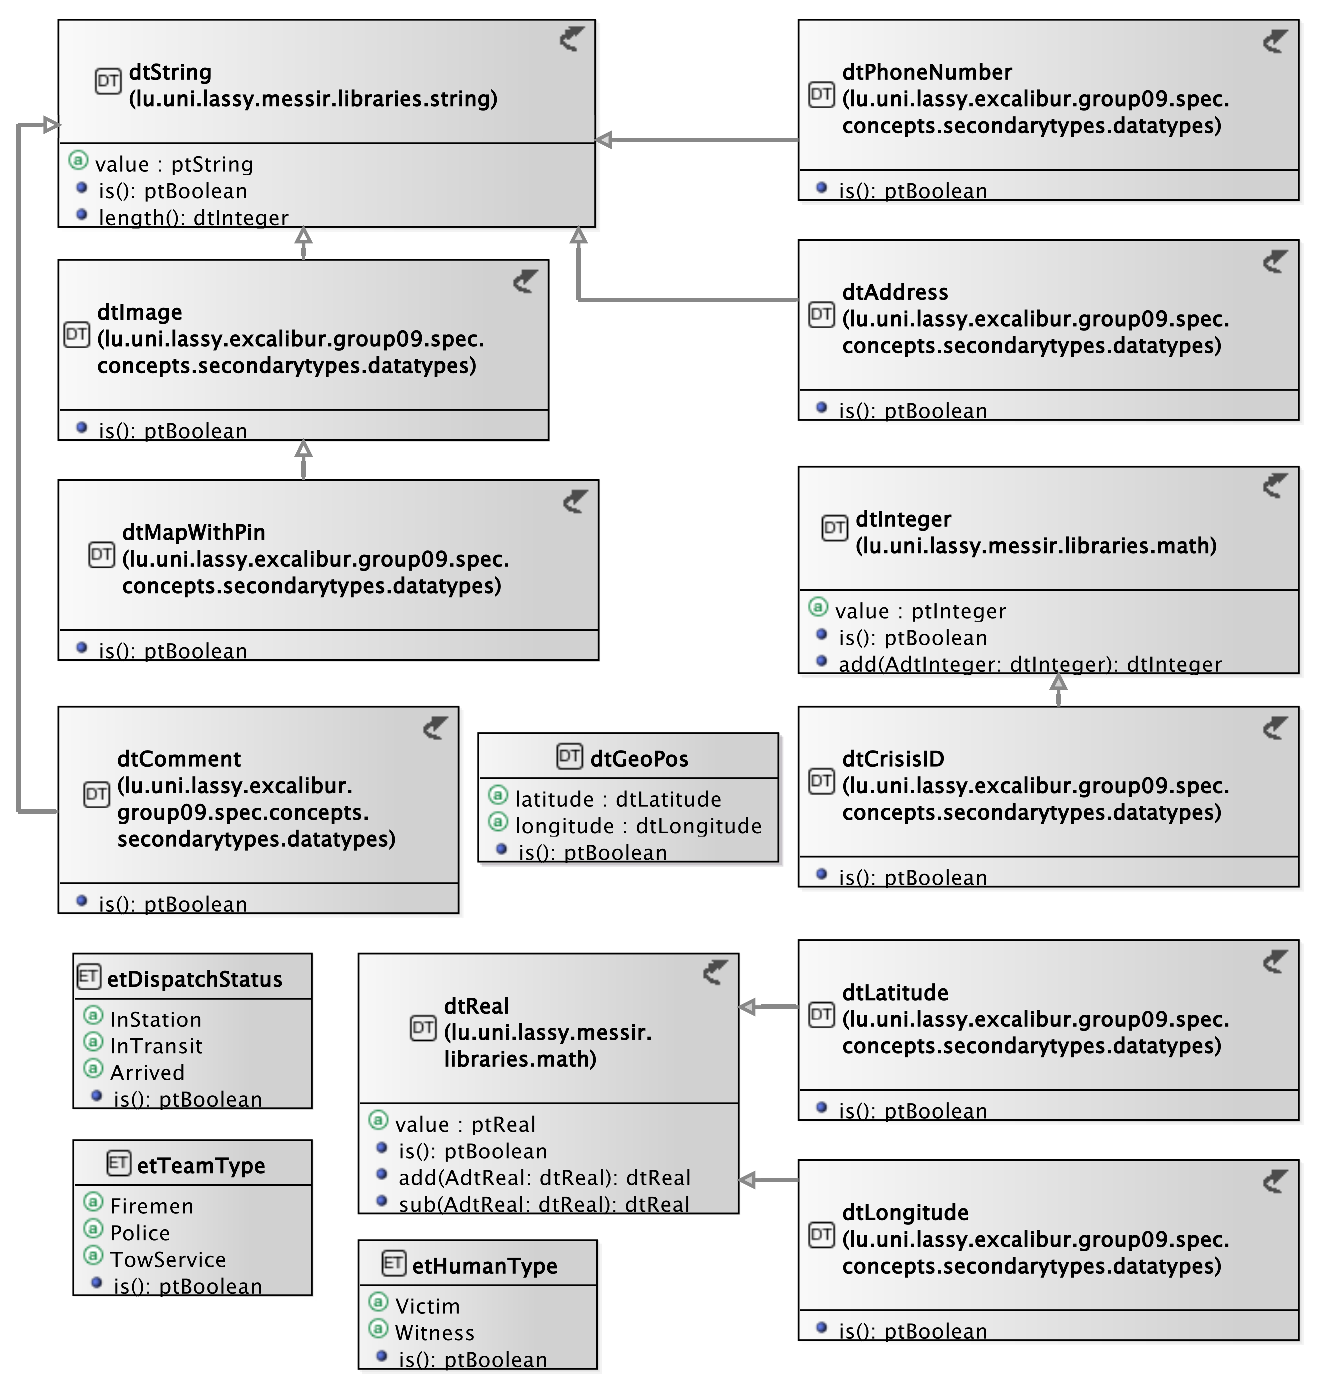
\includegraphics[
angle=0
,width=1.0\textwidth
]{./images-report-gen/concept-model/local/PrimaryTypes-Datatypes/15/cm-dt.eps}
\end{center}
\caption[Concept Model - PrimaryTypes-Datatypes local view 15 - View of all the datatypes]{Concept Model - PrimaryTypes-Datatypes local view 15. View of all the datatypes.}
\label{fig:lu.uni.lassy.excalibur.group09.spec-CM-view-local-PrimaryTypes-Datatypes-15}
\end{figure}
\vspace{0.5cm} 

\subsection{Local view 16}
\label{sec:lu.uni.lassy.excalibur.group09.spec-CM-view-local-PrimaryTypes-Datatypes-16}
Figure \ref{fig:lu.uni.lassy.excalibur.group09.spec-CM-view-local-PrimaryTypes-Datatypes-16} View of all the different modes for the coordinators/actors



\begin{figure}[htbp] 
\label{fig:lu.uni.lassy.excalibur.group09.spec-CM}
\begin{center}
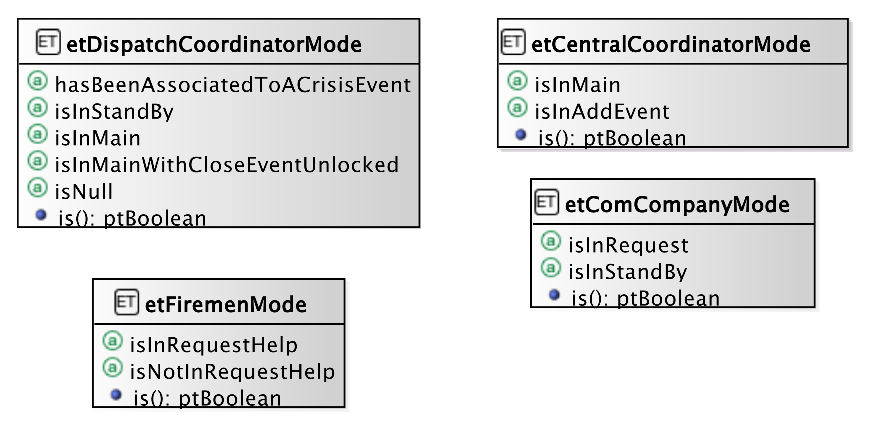
\includegraphics[
angle=0
,scale=0.80
]{./images-report-gen/concept-model/local/PrimaryTypes-Datatypes/16/cm-etModes.eps}
\end{center}
\caption[Concept Model - PrimaryTypes-Datatypes local view 16 - View of all the different modes for ]{Concept Model - PrimaryTypes-Datatypes local view 16. View of all the different modes for the coordinators/actors.}
\label{fig:lu.uni.lassy.excalibur.group09.spec-CM-view-local-PrimaryTypes-Datatypes-16}
\end{figure}
\vspace{0.5cm} 










\section{Concept Model Types Descriptions}
This section provides the textual descriptions of all the types defined in the concept model and that can be part of the graphical views provided.

\subsection{Primary types - Class types descriptions}




The table below is providing comments on the graphical views given for the class types of the primary types. Type logical operations are precisely specified in the operation model.

\begin{datadictionary}
\addheading{Classes}

\adddoublerow{ctComment}{A class containing a comment.}
\adddoubletwocolumnrow{attribute}{\msrcode{comment: dtComment}}{}
\adddoubletwocolumnrow{operation}{\msrcode{init(AComment:dtComment):ptBoolean}}{}
\adddoublerow{ctCrisisEvent}{A class containing the attributes identifying a crisis event.}
\adddoubletwocolumnrow{attribute}{\msrcode{id: dtCrisisID}}{}
\adddoubletwocolumnrow{attribute}{\msrcode{isLocationConfirmed: ptBoolean}}{}
\adddoubletwocolumnrow{attribute}{\msrcode{location: dtMapWithPin}}{}
\adddoubletwocolumnrow{operation}{\msrcode{init(Aid:dtCrisisID, Alocation:dtMapWithPin, AisLocationConfirmed:ptBoolean, Acomment:ptString, AgeoPos:dtGeoPos):ptBoolean}}{}
\adddoublerow{ctDispatchedCoordinator}{A class containing the attributes identifying a dispatched team.}
\adddoubletwocolumnrow{attribute}{\msrcode{status: etDispatchStatus}}{}
\adddoubletwocolumnrow{attribute}{\msrcode{type: etTeamType}}{}
\adddoubletwocolumnrow{operation}{\msrcode{init(Atype:etTeamType, Astatus:etDispatchStatus, AgeoPos:dtGeoPos):ptBoolean}}{}
\adddoublerow{ctHuman}{A class containing the attributes identifying an human.}
\adddoubletwocolumnrow{attribute}{\msrcode{id: dtPhoneNumber}}{}
\adddoubletwocolumnrow{attribute}{\msrcode{name: ptString}}{}
\adddoubletwocolumnrow{attribute}{\msrcode{type: etHumanType}}{}
\adddoubletwocolumnrow{operation}{\msrcode{init(Aid:dtPhoneNumber, Aname:ptString, Atype:etHumanType):ptBoolean}}{}
\adddoublerow{ctMapWithPin}{A class containing an image which is the map including the pins.}
\adddoubletwocolumnrow{attribute}{\msrcode{mapWithPin: dtMapWithPin}}{}
\adddoubletwocolumnrow{operation}{\msrcode{init(AmapWithPin:dtMapWithPin):ptBoolean}}{}
\adddoublerow{ctState}{used to model the system.}
\adddoubletwocolumnrow{attribute}{\msrcode{vpStarted: ptBoolean}}{}
\adddoubletwocolumnrow{operation}{\msrcode{init(ANextValueForAlertID:ptInteger, AvpStarted:ptBoolean):ptBoolean}}{}
\end{datadictionary}

\subsection{Primary types - Datatypes types descriptions}





The table below is providing comments on the graphical views given for the datatype types of the primary types.


\begin{datadictionary}
\addheading{Datatypes}

\adddoublerow{dtGeoPos}{Two Real numbers used to identify a geographical position on earth.}
\adddoubletwocolumnrow{attribute}{\msrcode{latitude: dtLatitude}}{}
\adddoubletwocolumnrow{attribute}{\msrcode{longitude: dtLongitude}}{}
\adddoubletwocolumnrow{operation}{\msrcode{is():ptBoolean}}{}
\end{datadictionary}


\begin{datadictionary}
\addheading{Enumerations}

\adddoublerow{etCentralCoordinatorMode}{Modes of the Central Coordinator to identify what operations he/she can do at what moment.}
\adddoubletwocolumnrow{operation}{\msrcode{is():ptBoolean}}{}
\adddoublerow{etComCompanyMode}{Modes of the Communication Company to identify what operations it can do at what moment.}
\adddoubletwocolumnrow{operation}{\msrcode{is():ptBoolean}}{}
\adddoublerow{etDispatchCoordinatorMode}{Modes of a dispatched Coordinator to identify what operations he/she can do at what moment.}
\adddoubletwocolumnrow{operation}{\msrcode{is():ptBoolean}}{}
\adddoublerow{etDispatchStatus}{A String used to identify a dispatch status.}
\adddoublerow{etFiremenMode}{Additional mode for the Firemen Coordinator to identify what operations he/she can do at what moment.}
\adddoubletwocolumnrow{operation}{\msrcode{is():ptBoolean}}{}
\adddoublerow{etHumanType}{A String used to identify an Human type.}
\adddoublerow{etTeamType}{A String used to identify a team type.}
\end{datadictionary}






\subsection{Primary types - Association types descriptions}




The table below is providing comments on the association types of the primary types.

\begin{associationtypes}
\addheading{Undirected associations}
\adddoublerow{assctCrisisEventctHuman}{Association of a crisis event to an human.}
\adddoublerow{assctDispatchedCoordinatoractAbstractDispatchCoordinator}{Association of a dispatched coordinator to an actor of the same type.}
\adddoublerow{assctDispatchedCoordinatorctCrisisEvent}{Association of a dispatched coordinator to a crisis event.}
\end{associationtypes}

\subsection{Primary types - Aggregation types descriptions}


There are no aggregation types for the primary types.


\subsubsection{Primary types - Composition types descriptions}



There are no composition types for the primary types.


\subsection{Secondary types - Class types descriptions}



There are no elements in this category in the system analysed.
		

\subsection{Secondary types - Datatypes types descriptions}





The table below is providing comments on the graphical views given for the datatype types of the secondary types.

\begin{datadictionary}
\addheading{Datatypes}

\adddoublerow{dtAddress}{A String used to identify an address.}
\addsingletwocolumnrow{extends}{dtString}
\adddoubletwocolumnrow{operation}{\msrcode{is():ptBoolean}}{}
\adddoublerow{dtCrisisID}{An Integer used to identify a crisis id.}
\addsingletwocolumnrow{extends}{dtInteger}
\adddoubletwocolumnrow{operation}{\msrcode{is():ptBoolean}}{}
\adddoublerow{dtImage}{A String used to identify an image.}
\addsingletwocolumnrow{extends}{dtString}
\adddoubletwocolumnrow{operation}{\msrcode{is():ptBoolean}}{}
\adddoublerow{dtLatitude}{used to define a latitude value of a geograpical positions on earth.}
\addsingletwocolumnrow{extends}{dtReal}
\adddoubletwocolumnrow{operation}{\msrcode{is():ptBoolean}}{}
\adddoublerow{dtLongitude}{used to define a longitude value of a geograpical positions on earth.}
\addsingletwocolumnrow{extends}{dtReal}
\adddoubletwocolumnrow{operation}{\msrcode{is():ptBoolean}}{}
\adddoublerow{dtMapWithPin}{An image which is a map including pins.}
\addsingletwocolumnrow{extends}{dtImage}
\adddoubletwocolumnrow{operation}{\msrcode{is():ptBoolean}}{}
\adddoublerow{dtPhoneNumber}{A String used to store a phone number.}
\addsingletwocolumnrow{extends}{dtString}
\adddoubletwocolumnrow{operation}{\msrcode{is():ptBoolean}}{}
\end{datadictionary}





\subsection{Secondary types - Association types descriptions}



There are no association types for the secondary types.



\subsection{Secondary types - Aggregation types descriptions}



There are no aggregation types for the secondary types.



\subsection{Secondary types - Composition types descriptions}



There are no composition types for the secondary types.



